
%(BEGIN_QUESTION)
% Copyright 2013, Tony R. Kuphaldt, released under the Creative Commons Attribution License (v 1.0)
% This means you may do almost anything with this work of mine, so long as you give me proper credit

An important concept in education is something called {\it schema}: the body of knowledge, expectations, and assumptions that someone uses to interpret any form of communication they are receiving, whether that communication be in the form of speech, text, or even something as abstract as art.  One does not approach an action-adventure novel in the same way or with the same expectations that one would approach instructions for filing tax returns with the IRS.  One does not interpret and appreciate a live jazz band in the same way they would interpret and appreciate choral music.  We have different schema for understanding and appreciating these different forms of communication, even if they occur in the same medium (e.g. printed text, or audible tones).

\vskip 10pt

Industrial system diagrams also have {\it schema} associated with them.  One does not interpret a P\&ID in the same manner that one interprets an electronic schematic or a block diagram, despite their many similarities.  This exercise will ask you to identify the meanings of similar symbols used in several types of diagrams, in order to expose some of the schema you have (or that you are in the process of building).

\vskip 10pt

Reference the following diagrams, and then answer the comparison/contrast questions that follow:

\vskip 10pt

\filbreak

\noindent
{\bf Schematic diagram of a relay circuit}
$$\includegraphics[width=15.5cm]{i02683x02.eps}$$

\filbreak

\noindent
{\bf Schematic diagram of a fuel tank level sensor circuit}
$$\includegraphics[width=15.5cm]{i02683x09.eps}$$


\filbreak

\noindent
{\bf Ladder diagram of a solenoid valve control circuit}
$$\includegraphics[width=15.5cm]{i02683x06.eps}$$

\filbreak

\noindent
{\bf P\&ID of a solvent storage tank}
$$\includegraphics[width=15.5cm]{i0006rx01.eps}$$

\filbreak

\noindent
{\bf Schematic diagram of a hydraulic valve control system}
$$\includegraphics[width=15.5cm]{i02683x01.eps}$$

\filbreak

\noindent
{\bf Schematic/pictorial diagram of a pressure transmitter}
$$\includegraphics[width=15.5cm]{i02683x03.eps}$$

\filbreak

\noindent
{\bf Pictorial diagram of an I/P transducer}
$$\includegraphics[width=15.5cm]{i02683x04.eps}$$

\filbreak

\noindent
{\bf Loop diagram of a compressor surge control system}
$$\includegraphics[width=15.5cm]{i02683x05.eps}$$

\filbreak

\noindent
{\bf Functional diagram of control loops}
$$\includegraphics[width=15.5cm]{i02683x07.eps}$$

\filbreak

\noindent
{\bf FOUNDATION Fieldbus function block diagram}
$$\includegraphics[width=15.5cm]{i02683x08.eps}$$



\vskip 10pt

\noindent
{\bf Questions:}
\begin{itemize}
\item{} Identify the meaning(s) of all {\it dashed lines} in these diagrams 
\item{} Identify the meaning(s) of all {\it arrows} in these diagrams 
\item{} Identify the meaning(s) of all {\it triangles} in these diagrams 
\item{} Identify the meaning(s) of all {\it boxes} in these diagrams 
\item{} Identify the meaning(s) of all {\it circles} in these diagrams 
\item{} Identify how directions of motion are indicated in each diagram (if at all)
\item{} Identify how sources of energy are indicated in each diagram (if at all)
\end{itemize}




\underbar{file i02683}
%(END_QUESTION)




%(BEGIN_ANSWER)



%(END_ANSWER)





%(BEGIN_NOTES)


%INDEX% Reading strategies: identifying schema in different diagram conventions 

%(END_NOTES)


